\subsection{Glyph: \glyph{Multimer}}
\label{sec:multimer}

As its name implies, a multimer is an aggregation of multiple identical or pseudo-identical entities held together by non-covalent bonds. Thus, they are distinguished from polymers by the fact that the latter involve covalent bonds, and should be represented by \glyph{macromolecules}. Here \emph{pseudo-identical} refers to the possibility that the entities differ chemically but retain some common global characteristic, such as a structure or function, and so can be considered identical within the context of the SBGN \PD.  An example of this are the homologous subunits in a hetero-oligomeric receptor. SBGN \PD accepts multimers of \glyph{simple chemical} (\sect{simpleChemical}), \glyph{macromolecule} (\sect{macromolecule}), \glyph{nucleic acid feature} (\sect{genetic}) or \glyph{complex} (\sect{complex}). A \glyph{multimer} is represented by two identical containers shifted horizontally and vertically and stacked one on top of the other as illustrated in \fig{multimer}.

\begin{figure}[H]
  \centering
  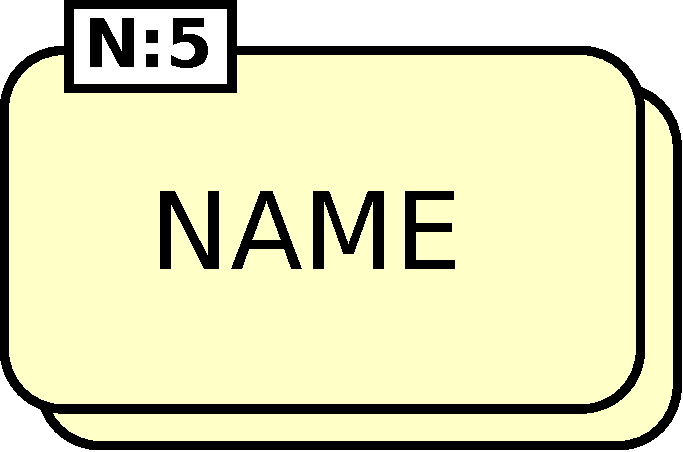
\includegraphics[scale = 0.3]{images/multimer}
  \caption{The \PD glyph for \glyph{multimer}. }
  \label{fig:multimer}
\end{figure}

Examples of \glyph{multimers} are presented in \fig{multimer-examples}.

\begin{figure}[H]
  \centering
  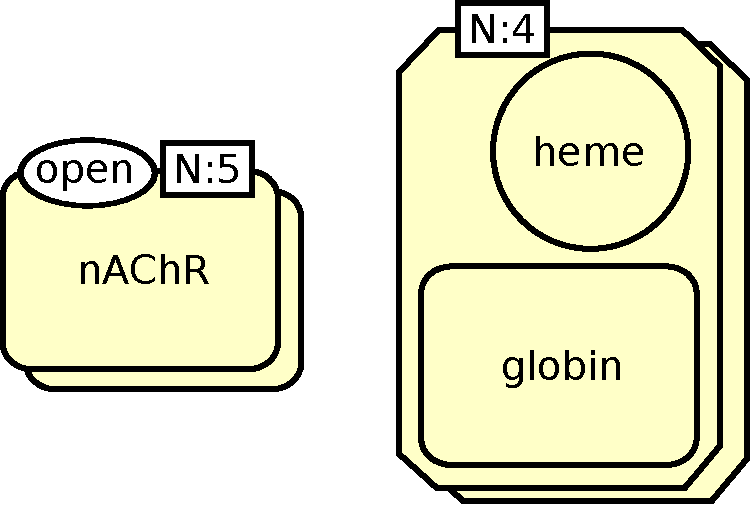
\includegraphics[scale = 0.5]{images/multimer-examples}
  \caption{Examples of \glyph{multimers}. From left to right: pentameric nicotinic receptor in the open state, tetramer of oxygenated globin.}
  \label{fig:multimer-examples}
\end{figure}